\documentclass[xcolor=dvipsnames]{beamer} \usepackage{beamerthemesplit}
\usecolortheme[named=OliveGreen]{structure} 

\useoutertheme{miniframes} 
\author{K Chahal, T Yang, J Zhou}
\title{36-350 Project Fall'13}

\usetheme{Berkeley}
\newcommand*\oldmacro{}%
\let\oldmacro\insertshorttitle%
\renewcommand*\insertshorttitle{%
  \oldmacro\hfill%
  \insertframenumber}
\setbeamertemplate{navigation symbols}{}

 \makeatletter
  \setbeamertemplate{sidebar \beamer@sidebarside}%{sidebar theme}
  {
    \beamer@tempdim=\beamer@sidebarwidth%
    \advance\beamer@tempdim by -6pt%
    \insertverticalnavigation{\beamer@sidebarwidth}%
    \vfill
    \ifx\beamer@sidebarside\beamer@lefttext%
    \else%
      \usebeamercolor{normal text}%
      \llap{\usebeamertemplate***{navigation symbols}\hskip0.1cm}%
      \vskip2pt%
    \fi%
  }%
\makeatother


\usepackage{amsthm,amssymb,amsmath}
\usepackage{bbm}
\usepackage{hyperref}
\usepackage{setspace} 
\usepackage[english]{babel}
\newcommand{\HRule}{\rule{\linewidth}{0.5mm}}
\usepackage{fancyref}
\usepackage{color}
\usepackage{caption}
\usepackage{subcaption} % for subfigures
\usepackage{booktabs} % for 'cleaner' tables
\newcommand{\ra}[1]{\renewcommand{\arraystretch}{#1}}
\usepackage{listings}
\usepackage{float}

\usepackage{etoolbox} % square bracket for \bordermatrix
\let\bbordermatrix\bordermatrix
\patchcmd{\bbordermatrix}{8.75}{4.75}{}{}
\patchcmd{\bbordermatrix}{\left(}{\left[}{}{}
\patchcmd{\bbordermatrix}{\right)}{\right]}{}{}


\begin{document}

\begin{frame}
    \title{Simulating Genome of \\ \emph{Dictyostelium discoideum} Using \\ $k^{th}$-Order Markov Chain Genetic Models}
    \author{Kairavi Chahal, Tony Yang, Julian Zhou}
    
    \institute{Department of Statistics \\
    Carnegie Mellon University}
    \maketitle
\end{frame}


\section{Introduction}
% intro to k-th order markov chain, transition matrices
\begin{frame}
	\frametitle{Chromosomes, DNA sequences, nucleotide bases}
	\begin{itemize}
		\item Soil-living amoeba, aka `slime mold' 
		\item Interested in simulating sequences of \emph{ATGC} 
	\end{itemize}

	\begin{figure}
	\centering
	\begin{subfigure}[b]{.22\textwidth}
	  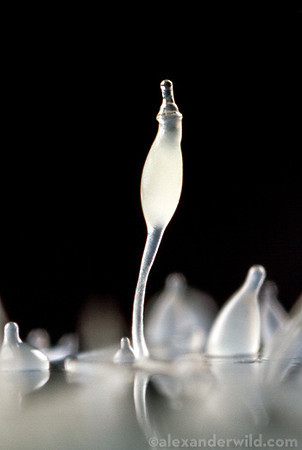
\includegraphics[width=\textwidth]{Dictyostelium5-M.jpg}\\
	  \tiny{Source: Alex Wild, Scientific American}
	  \label{fig:orgm}
	\end{subfigure}
	\begin{subfigure}[b]{.74\textwidth}
	  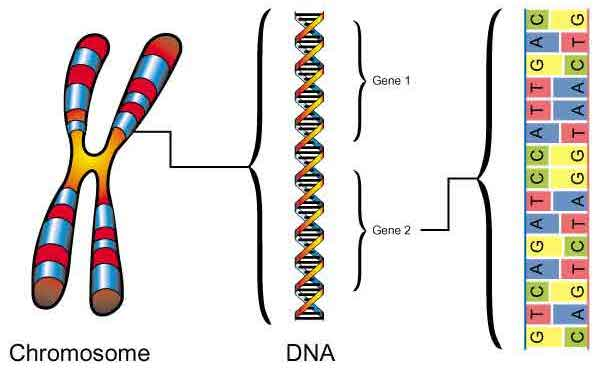
\includegraphics[width=\textwidth]{ChromgendnaLG.jpg}\\
	  \tiny{Source: Plant \& Soil Sciences eLibrary}
	  \label{fig:chrm}
	\end{subfigure}
	
	%\caption{}
	\label{fig:orgm_chrm}
	\end{figure}
\end{frame}	

\begin{frame}
	\frametitle{$k^{th}$-th Order Markov Chain}
	\begin{itemize}
		\item A single-stranded DNA sequence: $B_1,\;B_2,\;...,\;B_i$; $b=\{A,\;T,\;G,\;C\}$
		\item $P(B_i=b|B_{i-1},\;...,\;B_1)=P(B_i=b|B_{i-1},\;...,\;B_{i-k})$ \\
		\item i.e. $P(B_i=b)$ is \emph{conditionally independent} of \{$B_{i-k-1},\;...,\;B_1$\}, given \{$B_i,\;...,\;B_{i-k}\}$
	\end{itemize}
	
\end{frame}

\begin{frame}
	\frametitle{$k^{th}$-th Order Transition Matrix}
	\begin{itemize}
		\item Row: $(i-k)^{th}$ through $(i-t)^{th}$ bases - `prior sequence'
		\item Column: $i^{th}$ base
		\item Dimension: $4^k$x$4$
		\item Each row sums up to 1
		\item E.g. $2^{nd}$-order transition matrix based on original sequence in Chromosome 2\\
			\begin{center}
			\tiny{
					$
			\bbordermatrix{
			  ~ & A & C & G & T \cr 
			AA & 0.505 & 0.093 & 0.074 & 0.328 \cr
			AC & 0.420 & 0.245 & 0.054 & 0.282 \cr
			AG & 0.424 & 0.107 & 0.131 & 0.337 \cr
			AT & 0.310 & 0.127 & 0.119 & 0.445 \cr
			CA & 0.468 & 0.138 & 0.093 & 0.300 \cr
			CC & 0.612 & 0.116 & 0.045 & 0.227 \cr
			CG & 0.436 & 0.106 & 0.131 & 0.327 \cr
			CT & 0.277 & 0.152 & 0.151 & 0.419 \cr
			GA & 0.420 & 0.071 & 0.114 & 0.394 \cr
			GC & 0.462 & 0.142 & 0.065 & 0.332 \cr
			GG & 0.307 & 0.078 & 0.114 & 0.501 \cr
			GT & 0.290 & 0.080 & 0.191 & 0.439 \cr
			TA & 0.436 & 0.103 & 0.082 & 0.380 \cr
			TC & 0.484 & 0.135 & 0.066 & 0.316 \cr
			TG & 0.387 & 0.091 & 0.219 & 0.303 \cr
			TT & 0.262 & 0.100 & 0.135 & 0.503 \cr
			}$ }
			\end{center}
	\end{itemize}
\end{frame}

\section{Data}
\begin{frame}
	\frametitle{Reading in Data}
	
	\begin{center}
	\begin{raggedright}
	\tiny{
	\texttt{>DDB0169550 |Chromosomal Sequence| Chromosome: M position 1 to 55564}\\
	\texttt{AATGAAATAAAAAAAAACGAAAATAAAAAAAAATAATGACAATAATAGCAATAAGTATAA}\\
	\texttt{TGAATGTAGTGATAGGGATAGCAATATTAGGAGTAATATTAAGAAAGAAAATAATGCCGA}\\
	\texttt{ACCAAAAATTTCAAAGAATATTTATATTAGGAGTACAAGGAATACTAATAGTATTAAGTG} \\ }
	\end{raggedright}
	\end{center}

	\begin{itemize}
	\item Observe that the data is in \texttt{FASTA} format
	\item Function \texttt{read.fasta} in package \texttt{seqinr} reads such format
	
	\end{itemize}

\end{frame}


\begin{frame}
	\frametitle{Summary of Data}
	
	\begin{table}
	\centering
	\ra{1}
	%\caption{}
	\label{tab:data}
	\begin{tabular} {@{}rr@{}} 
	\toprule
	Chromosome & Length ($bases$)\\
	\midrule
	1 & $4,923,596$\\
	2 & $8,484,197$\\
	2F & $161,967$\\
	3 & $6,357,299$\\
	3F & $16,660$\\
	4 & $5,450,249$\\
	5 & $5,125,352$\\
	6 & $3,602,379$\\
	BF & $75,732$\\	
	M & $55,564$\\
	R & $85,150$\\
	\bottomrule
	\end{tabular} 
	\end{table}

\end{frame}


\section{Research Questions}

\begin{frame}
	\frametitle{Questions of Interest}
    \begin{itemize}
    \item How do simulation results change as $k$ changes?
    \item Do simulation results differ from one chromosome to another?
    \end{itemize}
\end{frame}

\begin{frame}
	\frametitle{Why not just concatenate the chromosomes?}
    \begin{itemize}
    	\item Doing so assumes that the starting sequence of one chromosome depends on the ending sequence of another
    	\item Doing so assumes that transition matrices will be similar for each chromosome
        \item Markov matrices for the whole genome and individual chromosomes may be different
        \item Order in which to join the chromosomes is unknown 
        \item Logistically, computing transition matrix and simulate the sequence for the entire genome would be overly time-consuming
    \end{itemize}
\end{frame}

\section{Algorithms}
\begin{frame}
	\frametitle{Overview of Our Code}
	\begin{figure}
        \centering
        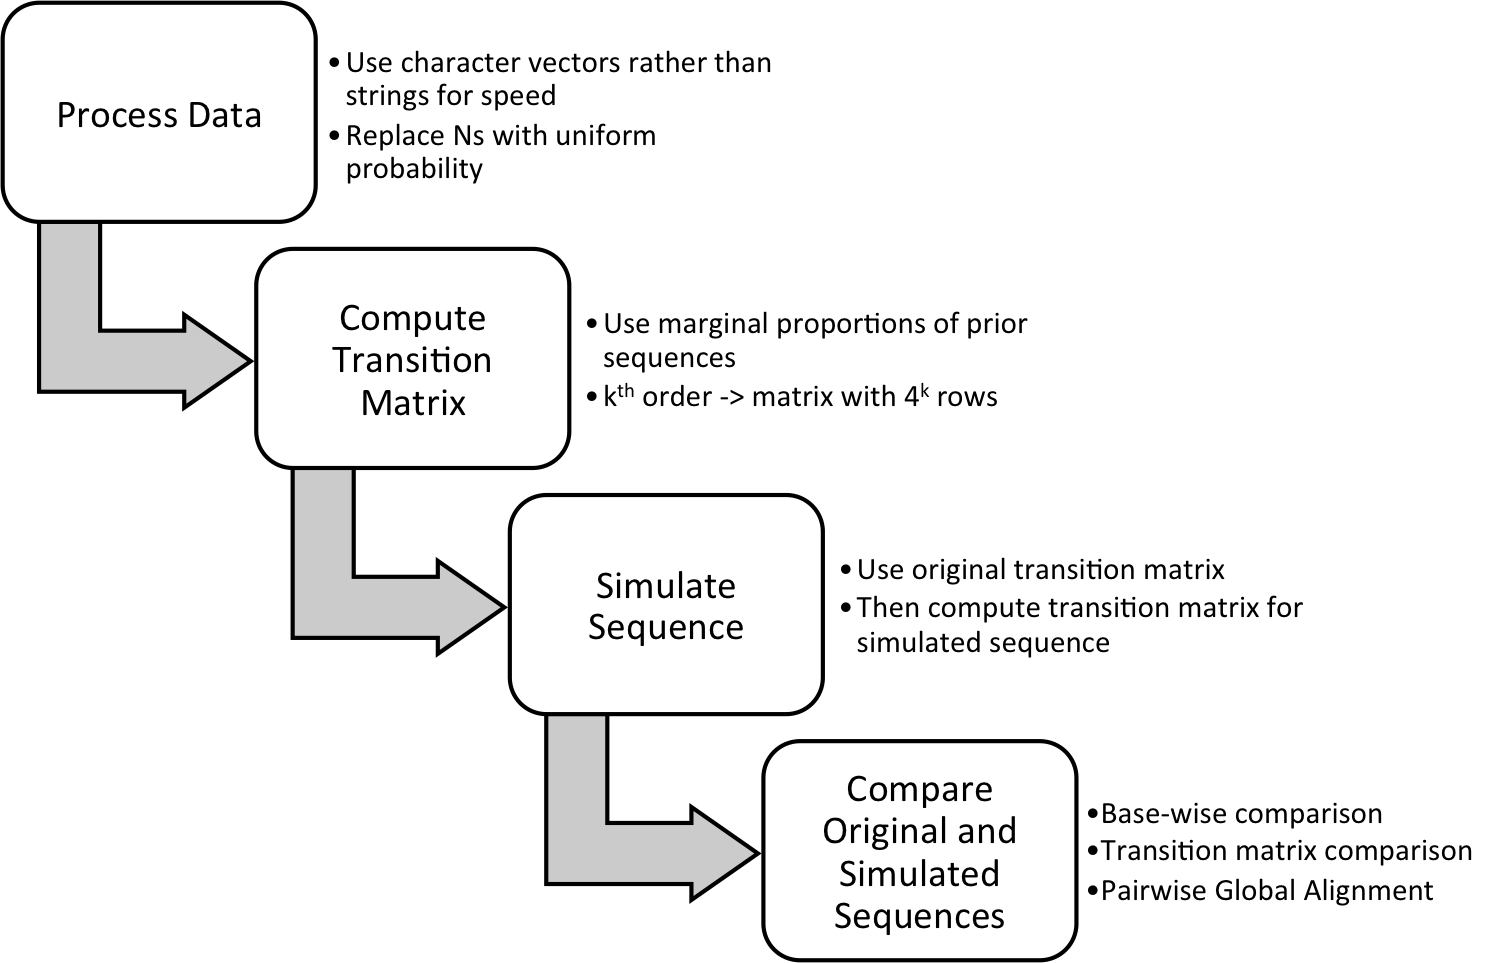
\includegraphics[scale=0.4]{algorithm_flowchart.png}
    \end{figure}
\end{frame}

\begin{frame}
	\frametitle{Replacing Ns}
    \begin{itemize}
    	\item \textbf{Idea:} replace the Ns with nucleotides using a uniform distribution
    	\item \textbf{Alternative Idea:} calculating a matrix of marginal probabilities based on the rest of the sequence, and then applying it to the sequence of Ns as a $0^{th}$ order
        \begin{itemize}
        	\item \textbf{Problem:} The marginal prob. matrix is inconsistent with the overall transition matrix
        \end{itemize}
	   	\item \textbf{Alternative Idea:} Drop all Ns
        \begin{itemize}
        	\item \textbf{Problem:} Will affect the transition matrix and results
        \end{itemize}

    \end{itemize}
\end{frame}

\begin{frame}
	\frametitle{Computing Transition Matrices}
    \begin{itemize}
    	\item Choose order $k$, and obtain all consecutive substrings of length k+1
        \item Group substrings by which nucleotide is in last (k+1th) position
        \item Count occurences of sequence of nucleotides in 1st to kth position within the four groups
        \item Divide each row by the sum of the row (ensures each row's probability is 1)
        \item If a row has all zeroes, then replace with all 0.25, since each combination is equally (un)likely
    \end{itemize}
\end{frame}



\begin{frame}
	\frametitle{Simulations}
    \begin{itemize}
    	\item Idea:
        \begin{itemize}
    		\item Take the first $k$ nucleotide bases as a starting point
        	\item Use the transition matrix to simulate the next base
        	\item Take the last $k$ nucleotide bases in the current simulated sequence, use transition matrix, repeat
        \end{itemize}
        \item 10 simulations per combination of chromosome \& order $k$ (ranging from 1 to 3)
        
    \end{itemize}
\end{frame}

\begin{frame}
	\frametitle{Why not convert nucleotides into codons?}
    \begin{itemize}
    	\item Codons are degenerate
        \item Without knowledge of where the \emph{coding} region begins, simply treating the first 3 bases as the starting codon could result in \emph{frameshift mutation}
        \begin{figure}
        \centering
        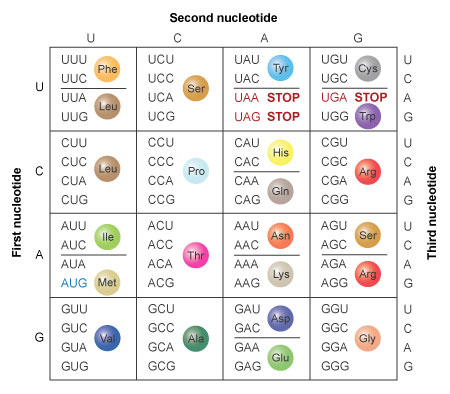
\includegraphics[scale=0.38]{EssGen1-5_genetic_code_0.jpg}
        \tiny{Source: Nature}
        \end{figure}
    \end{itemize}
\end{frame}

\subsection{Comparison}
\begin{frame}
	\frametitle{Base-wise Comparision}
	\begin{itemize}
		\item Number of exact matches
		\item Proportions of A, T, G, C (marginal probability distribution)
	\end{itemize}
\end{frame}

\begin{frame}
	\frametitle{Comparing Transition Matrices}
	\begin{itemize}
		\item $\mathbb{M}_{orig}$: transition matrix based on the original sequence
		\item $\mathbb{M}_{sim}$: transition matrix based on the osimulated sequence
		\item $\theta = \displaystyle{ \frac{ \sum_{i=1}^{4^k} \sum_{j=1}^{4} {|\mathbb{M}_{orig_{ij}}-\mathbb{M}_{sim_{ij}}|} }{4^{k+1}} }$
	\end{itemize}
\end{frame}

\begin{frame}
	\frametitle{Pairwise Global Alignment}
	\begin{itemize}
		\item  \emph{Needleman-Wunsch} algorithm (dynamic programming)
		\item Implemented by \texttt{pairwiseAlignment} in package \texttt{Biostrings} of Bioconductor
		\item Yields an optimal pairwise alignment score, based on a given scoring scheme
	\end{itemize}
\end{frame}

\begin{frame}
	\frametitle{Pairwise Global Alignment - Scoring Scheme}
	\begin{itemize}
		\item General guidelines
			\begin{itemize}
			\item If looking for closely related sequences, penalize mismatches/ gaps a lot
			\item Heavier penalty for a gap opening; smaller penalty for subsequent gap extensions
			\end{itemize}
		\item match$=+2$, mismatch$-2$, gap opening$=-5$, gap extension$=-2$
	\end{itemize}
	\insertframenumber
\end{frame}


\section{Results}


\section{Discussion}
\begin{frame}
	\frametitle{Possible Improvements to Algorithm/Code}
    \begin{itemize}
    	\item Represent bases with integers (0, 1, 2, 3) instead of characters ('a', 'c', 'g', 't'), since R processes them faster
        \item Use BLAST for comparison, which is faster and has a standardized result. But possibility of human-error when copying/pasting.
        \item Previously assumed transition matrices remain constant throughout. Could take into account of evolution of transition matrices, mutation rates, etc.
    \end{itemize}
\end{frame}

\begin{frame}
	\frametitle{threads of thought (temporary}
    \begin{itemize}
    \item 
    \item split/apply/combine - analyzing 11 chromosomes instead of 1 genome
    \end{itemize}
\end{frame}


\section{References}
\begin{frame}
	\frametitle{Acknowledgment}
	\begin{itemize}
		\item http://a-little-book-of-r-for-bioinformatics.readthedocs.org/en/latest/src/chapter1.html
		\item http://a-little-book-of-r-for-bioinformatics.readthedocs.org/en/latest/src/chapter4.html
		\item http://cran.r-project.org/web/packages/seqinr/seqinr.pdf
		\item http://tata-box-blog.blogspot.com/2012/04/introduction-to-markov-chains-and.html

	\end{itemize}

\end{frame}

\end{document}
